%=========================================================================
% (c) Michal Bidlo, Bohuslav Křena, 2008

%%%%%%%%%%%%%%%%%%%%%%%%%%%%%%%%%%%%%%%%%%%%%%%%%%%%%%%%%%%%%%%%%%%%%%%%%%%
%%%%%%%%%%%%%%%%%%%%%%%%%%%%%%%%%%%%%%%%%%%%%%%%%%%%%%%%%%%%%%%%%%%%%%%%%%%
%%%%%%%%%%%%%%%%%%%%%%%%%%%%%%%%%%%%%%%%%%%%%%%%%%%%%%%%%%%%%%%%%%%%%%%%%%%
%%%%%%%%%%%%%%%%%%%%%%%%%%%%%%%%%%%%%%%%%%%%%%%%%%%%%%%%%%%%%%%%%%%%%%%%%%%
\chapter{Úvod}

V~dnešnom svete je už možné previesť počítačový model do reálneho sveta vďaka 3D tlači. Táto tlač je ale pre mnohých stále príliš drahá. Modely Sliceforms sú tvorené len z~papiera, ktorý nie je taký drahý a pri skladaní jednotlivých plátkov poskytuje tvorcom potešenie a následne hrdosť na poskladané objekty.

Zadaním tejto práce bolo vytvoriť aplikáciu na tvorbu skladačiek známych ako Sliceforms. Táto aplikácia je vytvorená pomocou herného jadra Unity. 

Druhá kapitola sa zaoberá históriou modelov Sliceforms a ich skladaním. 
Tretia kapitola sa zaoberá matematickými a technickými prostriedkami. Kapitola sa začína popisom reprezentácie geometrických telies používaných v~počítačovej grafike. Nasledujú geometrické operácie, ktoré sú potrebné na tvorbu prierezov z~polygonálneho modela. Ďalej sa kapitola zaoberá herným jadrom Unity, pomocou ktorého je vytvorená výsledná aplikácia. V~závere tretej kapitoly je popísaný súborový formát OBJ, ktorý je v~vo výslednej aplikácii spracovávaný pri načítavaní polygonálneho modelu.
Štvrtá kapitola popisuje postup tvorby plátkov. Kapitola sa začína postupom tvorby prierezov a trianguláciou vzniknutých polygónov. Kapitola pokračuje popisom tvorby zárezov do plátkov a končí sa popisom ukladania finálneho produktu do súboru.
Piata kapitola detailne popisuje zvolené užívateľské rozhranie použité vo výslednej aplikácii a kláves používaných na ovládanie aplikácie.
Šiesta kapitola popisuje vyhodnotenie vytvoreného riešenia a obsahuje rady k~skladaniu.
V~poslednej siedmej kapitole je popísané možné pokračovanie projektu a o~jeho možnom vylepšení.


%V tejto práci sa zoznámime s modelmi Sliceforms a s algoritmom na ich tvorbu. 

%%%%%%%%%%%%%%%%%%%%%%%%%%%%%%%%%%%%%%%%%%%%%%%%%%%%%%%%%%%%%%%%%%%%%%%%%%%
%%%%%%%%%%%%%%%%%%%%%%%%%%%%%%%%%%%%%%%%%%%%%%%%%%%%%%%%%%%%%%%%%%%%%%%%%%%
%%%%%%%%%%%%%%%%%%%%%%%%%%%%%%%%%%%%%%%%%%%%%%%%%%%%%%%%%%%%%%%%%%%%%%%%%%%
%%%%%%%%%%%%%%%%%%%%%%%%%%%%%%%%%%%%%%%%%%%%%%%%%%%%%%%%%%%%%%%%%%%%%%%%%%%
\chapter{Motivácia pre riešenú úlohu}

V~dnešnej dobe je niekoľko spôsobov ako vytvoriť skladačky Sliceforms. Jednou z~nich je \textit{Slicer for Fusion 360}\footnote{https://apps.autodesk.com/FUSION/en/Detail/Index?id=8699194120463301363} od firmy Autodesk, ktorá bola nahradená za ukončenú aplikáciu 123D Make na začiatku roka 2017. Táto aplikácia umožňuje vytvoriť prierezy z~vybraného objektu a zobraziť ich v~rovine. Zároveň umožňuje aj jednotlivé rezy ľubovoľne posúvať a tým zdokonaliť navrhnutý model.
%$$$$$$$$$$$$$$$$$$$$$$$$$$$$$$$$$$$$$$$$$$$$$$$$$$$$$$$$$$$$$$$$$$$$$$$$$$$$$$
\section{Prierezový model Sliceform}

\begin{quotation} \textit{
\uv{Obrázky modelov Sliceform neukážu ich celú krásu. Iba vytváraním a fyzickým zaobchádzaním s~modelmi je možné plne oceniť ich skutočné dynamické vlastnosti,} }John Sharp \cite{sharp1995sliceforms}.
\end{quotation}



%\uv{Obrázky modelov sliceform neukážu ich celú krásu. Iba vytváraním a fyzickým zaobchádzaním s modelmi je možné plne oceniť ich skutočné dynamické vlastnosti.} John Sharp\cite{sharp1995sliceforms}

Trojrozmerné objekty nazývané modely Sliceform majú vytvorenú formu z~dvoch paralelne pretínajúcich sa sád plátov. Väčšina modelov Sliceform sa neustále deformuje, a to do dvoch plochých tvarov \cite{sharp1995sliceforms}.





Olaus Henrici je matematik, ktorý na konci 19. storočia navrhol techniku modelov Sliceform. Modely, ktoré vytvoril, boli tvorené prierezmi štvorcových plôch \cite{johnsharp2010assemble}.
Nemecká firma Martin Schilling predávala modely, ktoré môžeme vidieť na obrázku \ref{fig:MartinSchilling}. Tieto modely navrhol Alexander von Brill v~roku 1874 a boli inšpirované modelmi, ktoré Henrici poslal na stretnutie matematikov v~Göttingenu. Tieto lepenkové modely neboli také robustné ako drevené alebo plastové ale boli podstatne lacnejšie \cite{brill}.

John Sharp neskôr rozšíril modely na rôzne povrchy a polyhedrony a pomenoval ich pod názvom Sliceforms.


\begin{figure}[H]
\centering
\tmpframe{\includegraphics[width=0.6\linewidth]{obrazky-figures/teoria/MartinSchilling.pdf}}
\caption{Modely predávané firmou Martin Schilling.  Zdroj: \cite{kerrycue2013}
%\protect\footnotemark
} 
\label{fig:MartinSchilling}
\end{figure}
%\footnotetext{https://mathspig.wordpress.com/2013/04/09/3-ellipsoid-collipsoid/}
%\todo{davat aj najdeny obrazok ako citaciu ked nebol pouzity ziadny text?}

\subsection{Skladanie modelov Sliceforms}
Pred začatím skladania je najprv treba vystrihnúť všetky zárezy. Tieto zárezy je nutné vystrihnúť zastrihnutím pri vyznačenom záreze z~oboch strán.
Tým vznikne tenký vlások, ako môžeme vidieť na obrázku \ref{fig:zastrihovanie}, ktorý sa dá pomocou nechtov vybrať a vytvoriť tak dostatočne široký otvor na vkladanie kolmých plátkov. Tento otvor ale nemôže byť príliš široký, lebo model nebude pevne držať a rozpadne sa \cite{johnsharp2010assemble}.
\begin{figure}[H]
\centering
\tmpframe{\includegraphics[width=0.35\linewidth]{obrazky-figures/zarezy2x.pdf}}
\caption{Odporúčané zastrihovanie do prierezov. Zdroj:~\protect\cite{johnsharp2010assemble}}\label{fig:zastrihovanie}
\end{figure}


Na poskladanie skladačky Sliceforms je potrebné si zoradiť jednotlivé prierezy podľa numerickej postupnosti -- najmenšie číslo dole a navyššie hore. Skladanie dvoch kolmých plátov do seba je zobrazené na obrázku \ref{fig:vkladanie}.
\begin{figure}[H]
\centering
\tmpframe{\includegraphics[height=0.37\linewidth]{obrazky-figures/Skladanie/vkladanie.pdf}}
\caption{Spojenie dvoch kolmých rezov. Zdroj:~\protect\cite{johnsharp2010assemble}}
\label{fig:vkladanie}
\end{figure}

Je viacero možností ako poskladať model Sliceform. Inšpirovať sa je možné niektorov z~následujúcich metód \cite{sharp1995sliceforms}: 
%\todo{DONE Citace je součást věty, takže musí být ještě před koncovým interpunkčním znaménkem (tečkoku, dvojtečkou, \dots)}
\begin{description}
\item[Metóda 1:] Najprv vložíme do stredného plátku X všetky Y-ové plátky a potom prevrátime celý model a postupne od vloženého stredného plátku vkladáme ďaľšie X-ové plátky.
\item[Metóda 2:] Najprv si spojíme prostredné plátky z~osí X a Y a potom postupne striedavo vkladáme ďaľšie plátky z~jednotlivých osí a prevraciame model. Táto metóda je jednoduchšia, keďže pri vkladaní vnútornejších plátkov je ešte menší počet kolmých plátkov. A~pri vkladaní posledných plátkov je už model dostatočne stabilný.
\end{description}

\begin{figure}[H]
\centering
\tmpframe{\includegraphics[height=0.38\linewidth]{obrazky-figures/Skladanie/Skladanie-najprvX.png}}\quad
\tmpframe{\includegraphics[height=0.38\linewidth]{obrazky-figures/Skladanie/Skladanie-postupne.png}}
\caption{Dve varianty skladania. \textbf{Vľavo} je metóda vloženia všetkých plátkov z~jednej osi do stredného plátku kolmej osi a \textbf{vpravo} je metóda postupného striedavého vkladania plátkov. }\label{fig:skladanie}
\end{figure}


%%%%%%%%%%%%%%%%%%%%%%%%%%%%%%%%%%%%%%%%%%%%%%%%%%%%%%%%%%%%%%%%%%%%%%%%%%%
%%%%%%%%%%%%%%%%%%%%%%%%%%%%%%%%%%%%%%%%%%%%%%%%%%%%%%%%%%%%%%%%%%%%%%%%%%%
%%%%%%%%%%%%%%%%%%%%%%%%%%%%%%%%%%%%%%%%%%%%%%%%%%%%%%%%%%%%%%%%%%%%%%%%%%%
%%%%%%%%%%%%%%%%%%%%%%%%%%%%%%%%%%%%%%%%%%%%%%%%%%%%%%%%%%%%%%%%%%%%%%%%%%%
\chapter{Použité matematické a technické prostriedky}
%$$$$$$$$$$$$$$$$$$$$$$$$$$$$$$$$$$$$$$$$$$$$$$$$$$$$$$$$$$$$$$$$$$$$$$$$$$$$$$
\section{Reprezentacia geometrických telies v~počítačovej grafike}


Veľa počítačových objektov, ktoré sa nachádzajú v~trojrozmernom priestore majú charakter telesa. Tieto objekty pripomínajú reálne hmotné telesá, ktoré prirodzene nadobúdajú určitý objem.
Každé teleso sa skladá z~množiny vnútorných bodov a množiny hraničných bodov. Pri vnútornom bode sa nachádza aspoň jeden vnútorný a prípadne aj hraničný bod. Pri každom hraničnom bode sa nachádza aspoň jeden vnútorný, vonkajší a ďaľší hraničný bod. Všetky tieto tri množiny sú navzájom disjunktné. 
Z~uvedeného vyplýva, že sem nepatria objekty ako sú úsečky a krivky v~priestore, časti rovín a všeobecné plochy, keďže tieto objekty neobsahujú žiadne vnútorné body \cite{modernipocitacovagrafika}.

Hlavným stavebným prvkom v~počítačovej grafike je trojuholník, a to práve vďaka svojim dobrým vlastnostiam. Je vždy konvexný a vždy leží celý v~jednej rovine, narozdiel od všeobecných mnohouholníkov. Pre trojuholníky existujú veľmi rýchle algoritmy pre vyplňovanie a jeho zobrazovanie je podporované grafikým procesorom.

Množinu trojuholníkov, ktorá zdieľa svoje hrany, nazývame sieťou (triangle mesh). Dátovú štruktúru, ktorá popisuje sieť, môžeme rozdeliť  do dvoch častí a to:
\begin{description}
\item[geometrická časť:] Zaznamenáva súradnice vrcholov trojuholníka.
\item[topologická časť:] Uchováva údaje o~vrcholoch tvoriace trojuholník. 
\end{description}
Toto rozdelenie umožňuje vykonávať geometrické transformácie so zmenou súradnic vrcholov len so zmenou geometrickej časti a nie je potrebná zmena topologickej časti \cite{modernipocitacovagrafika}.

\subsection{T-vrcholy} \label{Sec:TVrchol}
Sieť trojuholníkov má aj svoju nevýhodu, a tou je geometrický alias, ktorý sa prejavuje pri zmene mierky. Najčastejší jav ktorý to spôsobuje sa nazýva T-vchol. Tento jav je možné vidieť na obrázku ~\ref{fig:TVrchol}. 
Pri pozícii vrchola nastáva numerická chyba, ktorá je dôsledkom toho, že pamäť počítača nie je nekonečná. Táto malá vzdialenosť zapríčiňuje, že zo vzdialenosti je vidieť objekt spojený, ale po priblížení je vidieť v~objekte dieru.
T-vrcholy často vznikajú pri priebežnej zmene úrovne detailov alebo pri spojení dvoch sietí trojuholníkov \cite{modernipocitacovagrafika}.

\begin{figure}[!h]
\centering
\tmpframe{\includegraphics[height=0.35\linewidth]{obrazky-figures/teoria/TVrchol.pdf}}
\caption{Na obrázku vidieť roztrhnutie siete pri T-vrchole, ktoré vytvára v~objekte dieru.}
\label{fig:TVrchol}
\end{figure}


\subsection{Manifoldy}
Ako bolo spomenuté vyššie, objekt je tvorený vnútornými a hraničnými bodmi. Táto reprezentácia ale nie je úplne vhodná, pretože popisuje aj také objekty, ktoré sa nedajú v~skutočnom svete vytvoriť.
Pojem manifold sa zaviedol práve pre také prípady, kedy je možné objekt vytvoriť aj v~skutočnom svete. Objekt, ktorý sa nedá vytvoriť sa nazýva nonmanifold. Príklad takéhoto objektu s~možným riešením prevodu na manifold môžeme vidieť na obrázku \ref{fig:nonmanifold}. Vo všeobecnosti môžeme povedať, že manifold je objekt, ktorého každá hrana spája práve dve plochy \cite{modernipocitacovagrafika}.

\begin{figure}[!h]
\centering
\tmpframe{\includegraphics[height=0.4\linewidth]{obrazky-figures/teoria/nonmanifold.pdf}}
\caption{Nonmanifold a dve možnosti jeho prevodu na manifold.  Zdroj:~\protect\cite{modernipocitacovagrafika}}
\label{fig:nonmanifold}
\end{figure}
%$$$$$$$$$$$$$$$$$$$$$$$$$$$$$$$$$$$$$$$$$$$$$$$$$$$$$$$$$$$$$$$$$$$$$$$$$$$$$$
\section{Potrebné geometrické operácie}
Na tvorbu plátkov na vystrihovačky Sliceforms bolo potrebné využiť niektoré geometrické operácie s~úsečkou a plochou. Tieto operácie budú následovne popísané v~tejto sekcii.

%%%%%%%%%%%%%%%%%%%%%%
\subsection{Vzdialenosť bodu od roviny}\label{Sec:Vzdialenost}

Vzdialenosť bodu od roviny sa vypočíta pomocou vzorca (\ref{eqn:vzdialenost}), kde sa premietne vektor $\overrightarrow{w}$ na normálu plochy $\overrightarrow{N_{p}}$.
Ak vzdialenosť bodov $P_{1}$ a $P_{2}$  úsečky $U$ je od roviny $R$ rovná nule ($d=0$), dá sa povedať, že úsečka $U$ leží na rovine $R$.

\begin{equation}
d = \overrightarrow{w}\cdot \overrightarrow{N_{p}}
\label{eqn:vzdialenost}
\end{equation}


\begin{figure}[H]
\centering
\tmpframe{\includegraphics[height=0.25\linewidth]{obrazky-figures/Geometricke_operacie/DistancePointFromPlane.pdf}}
\caption{Vzdialenosť bodu od roviny.}
\label{fig:distancePointFromPlane}
\end{figure}



%%%%%%%%%%%%%%%%%%%%%%%%%%
\subsection{Priesečník úsečky a roviny}


Bod pretnutia úsečky a roviny sa vypočíta pomocou vzorca (\ref{eqn:priesecnik2}). Pomocou tohto vzorca sa dostane vzdialenosť $\left | s \right |$, ktorá keď sa vynásobí normálou úsečky vznikne vektor~$\overrightarrow{s}$, ktorý sa pripočíta k~bodu $P_{1}$. Takto sa získa výsledná pozícia bodu pretnutia. Keďže tento výpočet zistuje bod pretnutia aj mimo úsečky $[P_{1}, P_{2}]$, je potrebné zistiť, či sa získaný bod aj skutočne nachádza medzi bodmi $P_{1}$ a $P_{2}$.
Ak je skalárny súčin vektorov $\overrightarrow{N_{L}}$ a $\overrightarrow{N_{p}}$ rovný nule znamená, že je úsečka rovnobežná s~rovinou.

\begin{equation}
\left | s \right |= \frac{\overrightarrow{w}\cdot \overrightarrow{N_{p}}}{\overrightarrow{N_{L}} \cdot \overrightarrow{N_{p}}}
\label{eqn:priesecnik1}
\end{equation}

\begin{equation}
P_{i} = P_{1} + \left | s \right | \times \overrightarrow{N_{L}}
\label{eqn:priesecnik2}
\end{equation}



\begin{figure}[H]
\centering
\tmpframe{\includegraphics[height=0.4\linewidth]{obrazky-figures/Geometricke_operacie/Intersect.pdf}}
\caption{Priesečník úsečky a roviny.}
\label{fig:Intersect}
\end{figure}


%$$$$$$$$$$$$$$$$$$$$$$$$$$$$$$$$$$$$$$$$$$$$$$$$$$$$$$$$$$$$$$$$$$$$$$$$$$$$$$
\section{Herný engine Unity}

Herný engine (herné jadro) je špecializovaný softvér na vytváranie nielen hier, ale aj rôznych aplikácií. Kedysi boli herné jadrá veľmi drahé a komplikované, a preto boli dostupné iba pre veľké štúdia. V~dnešnej dobe sú ale jednoduchšie a prístupné aj pre jednotlivcov. Jeden z~najrozšírenejších herných jadier je Unity. Unity je používaný rozmanitou komunitou vývojárov ako sú študenti a fanatici, ale aj mnohými organizáciami, ktoré používajú Unity na vývoj hier \cite{smith2013unity}.

Herný engine Unity pracuje so skriptami, ktoré môžu byť napísané v~jazyku Javascript alebo v~jazyku C\#.
Pomocou týchto skriptov sa ovládajú jednotlivé herné objekty. Tieto skripty sú spolu s~materiálmi a modelmi uložené v~priečinku Assets.


Výsledná aplikácia v~Unity je multiplatformová, stačí iba pri vytváraní aplikácie zvoliť cielenú platformu.

Prostredie Unity je rozdelené na \cite{smith2013unity}:
\begin{description}
\item[Scene] (Scéna):
Používa sa na výber herných objektov a navigáciu.
\item[Game] (Hra):
Táto časť je na testovanie aplikácie a umožňuje rovnaký pohľad na aplikáciu ako bude mať užívateľ.
\item[Hierarchy] (Hierarchia):
Zobrazuje herné objekty ako Herné objekty sú zobrazené v~stromovej štruktúre. 
\item[Project] (Projekt):
Táto časť obsahuje assety ako sú skripty, textúry a modely.
\item[Inspector] (Inšpektor):
Pomocou inšpektora je možné nastavovať herné objekty a komponenty, ktoré sú k~nemu pripojené.
\item[Toolbar] (Panel nástrojov):
Obsahuje transformačné nástroje a nástroje na spúštanie aplikácie.
\item[Menu] (Menu):
Umožňuje prístup k~rôznym príkazom, ktoré zahrňujú vytvorenie herného objektu, komponenty alebo zobrazenie manuálu.
\end{description}


\begin{figure}[H]
\centering
\tmpframe{\includegraphics[width=0.7\linewidth]{obrazky-figures/Unity.png}}
\caption{Prostredie herného jadra Unity. Zdroj: \cite{smith2013unity} }
\label{prostredieUnity}
\end{figure}


\section{Formát OBJ}

Keďže herný engine Unity neumožnuje natívne nahratie modelu počas behu aplikácie, bolo nutné sa zaoberať aj touto záležitosťou a vytvoriť aspoň jednoduchý spôsob pre import 3D modelu.
Rozhodol som sa pre súborový formát {\tt OBJ}, kvôli jeho dostupnosti a zároveň jednoduchosti pri spracovaní. 

OBJ je geometrický súborový formát, ktorý bol vytvorený spoločnosťou Wavefront Technologies pre ich animačný nástroj Advanced Visualizer. Tento súborový formát je v~súčastnosti verejne prístupný a bol prevzatý aj ďaľšími firmami, ktoré sa zaoberajú tvorbou 3D grafických aplikácií a stal sa jedným z~najpopulárnejších formátov pre popis 3D modelov.

Tento súborový formát je jednoduchý dátový formát, ktorý reprezentuje 3D polygonálne modely a je uložený ako prostý text. 3D polygonálne modely sú definované pomocou pozície jednotlivých vrcholov, súradnice textúry na vrchole, normály vertexu, a plochou (face), ktorá tvorí jednotlivé polygóny, a je definovaná ako list bodov, textúr a normál.

\begin{description}
\item[Názov objektu:] (object name)

{\color[HTML]{991212}\texttt{o \textit{názov}}}


V~jednom súbore môže byť uložených aj viac objektov. Toho sa dá docieliť pomocou tohto elementu. Tento element združuje prvky, ktoré sú po ňom následne definované.

\item[Komentár:] (comment)

\texttt{\color[HTML]{991212} \# \textit{komentár}}

Riadok začínajúci sa znakom \# sa vždy ignoruje. Ide o~riadok s~komentárom, ktorý zvyčajne obsahuje informácie o~programe, pomocou ktorého bol súbor vytvorený. Obvykle tiež obsahuje aj počet vrcholov alebo plôch, ktoré sú v~objekte použité.

\item[Vrchol:] (vertex)

\texttt{\color[HTML]{991212}  v~\textit{x y z}}

Vrcholy objektu sú označované znakom {\tt v}. Špecifukujú geometrické vrcholy a ich x, y a z~koordináty. Tieto koordináty sa zapisujú ako čísla s~plávajúcou desatinnou čiarkou.

\item[Plocha:] (face)

\texttt{\color[HTML]{991212}  f 
\textit{v1}[/[\textit{vt1}][/\textit{vn1}]] 
\textit{v2}[/[\textit{vt2}][/\textit{vn2}]] 
\textit{v3}[/[\textit{vt3}][/\textit{vn3}]] ...}

{\tt f} označuje plochu.
Plochy sa skladajú z~troch alebo viac trojíc čísel špecifikujúce číslo geometrického vrchola {\tt v}, textúry vrchola {\tt vt} a normály vrchola {\tt vn}. 
Textúra vrchola a normála vrchola sú nepovinné parametre. Táto trojica čísiel je oddelená pomocou znaku {\tt /}.
\end{description}
Ďalšie možnosti, ktoré formát {\tt OBJ} ponúka sú zhrnuté v~manuále \cite{objmanual:1}.


\pagebreak
Ukážka jednoduchej polygonálnej kocky vo formáte OBJ vytvorená iba pomocou vertexov a plôch:
\begin{framed}
{
\noindent
\# kocka.obj \\
o~kocka \\
v~1.000000 -1.000000 -1.000000\\
v~1.000000 -1.000000 1.000000\\
v~-1.000000 -1.000000 1.000000\\
v~-1.000000 -1.000000 -1.000000\\
v~1.000000 1.000000 -1.000000\\
v~1.000000 1.000000 1.000000\\
v~-1.000000 1.000000 1.000000\\
v~-1.000000 1.000000 -1.000000\\
f 5 1 4\\
f 5 4 8\\
f 3 7 8\\
f 3 8 4\\
f 2 6 3\\
f 6 7 3\\
f 1 5 2\\
f 5 6 2\\
f 5 8 6\\
f 8 7 6\\
f 1 2 3\\
f 1 3 4
}
\end{framed}

%%%%%%%%%%%%%%%%%%%%%%%%%%%%%%%%%%%%%%%%%%%%%%%%%%%%%%%%%%%%%%%%%%%%%%%%%%%
%%%%%%%%%%%%%%%%%%%%%%%%%%%%%%%%%%%%%%%%%%%%%%%%%%%%%%%%%%%%%%%%%%%%%%%%%%%
%%%%%%%%%%%%%%%%%%%%%%%%%%%%%%Kapitola 4%%%%%%%%%%%%%%%%%%%%%%%%%%%%%%%%%%%
%%%%%%%%%%%%%%%%%%%%%%%%%%%%%%%%%%%%%%%%%%%%%%%%%%%%%%%%%%%%%%%%%%%%%%%%%%%
\chapter{Navrhnuté riešenie generovania prierezov}
Pred začatím tvorby prierezov je potrebné načítaný objekt normalizovať, teda zmeniť jeho veľkosť tak, že najväčšia vzdialenosť v~niektorej osi bude rovná jedna.
%, aby sa vošiel do kocky s veľkosťou strany $1$.
Tento objekt sa ale nemusí nachádzať na správnej pozícii, preto je treba jeho stred umiestniť na bod $[0,0,0]$.

Generovanie prierezov prebieha pre každú os zvlášť a to v~dvoch fázach. Generovanie sa začína od stredu a postupným pripočítavaním vektoru posunu k~reznej ploche sa generujú ďaľšie prierezy. Tento proces trvá až pokiaľ nedôjde k~bodu, kde rez nepretne plochu objektu. V~tomto bode sa generovanie presunie na zápornú časť objektu, a tam sa znova začnú generovať prierezy ale tentoraz sa už vektor posunu odpočítava.

%$$$$$$$$$$$$$$$$$$$$$$$$$$$$$$$$$4.1$$$$$$$$$$$$$$$$$$$$$$$$$$$$$$$$$$$$$$
\section{Postup generovania prierezov}
Prierezy generujeme tak, že prechádzame všetky trojuholníky v~polygonálnom modele a testujeme na pretnutie reznou rovinou. Ak je trojuholník pretnutý, zaznamenáme úsečku, v~ktorej sme ho pretli. To sa deje na základe algoritmu \ref{FindCollides}. Tento algoritmus najprv zistí pozície bodov trojuholníku a následne zistuje, ktoré úsečky medzi bodmi tojuholníka sa pretínajú s~reznou rovinou. Sú 4 možnosti ako môže rovina prechádzať cez trojuholník. Tieto možnosti sú zobrazené na obrázku \ref{FindCollidesPic}.

Vo variante $A$ a variante $B$ pretína rovina úsečky $[A,C]$ a $[B,C]$. V~možnosti $A$ sa priesečník týchto dvoch úsečiek s~rovinou nachádza práve v~bode $C$. Tieto dve varianty berem ako rovnocenné, keďže nám pridanie jedného bodu viacnásobne výsledný tvar nijak neovplivňuje a po nájdení všetkých bodov a následnom spojení sa zredukujú body, ktoré sa nachádzajú na približne rovnakej súradnici.
Pri variante $C$ prechádza rovina cez všetky tri úsečky. Úsečky $[A,C]$ a $[B,C]$ pretína práve v~jednom bode $C$ a úsečku $[A,B]$ pretína niekde medzi bodmi $A$ a $B$.Vo variante D rovina leží na úsečke $[B,C]$. Je pravda, že prechádza tiež cez úsečky $[A,B]$ a $[C,A]$ ale kedže túto variantu -- ako je vidno v~algoritme \ref{FindCollides} -- testujem ako prvú, tak sa zaznamenajú iba body $B$ a $C$.
Tento proces sa opakuje pre každý trojuholník v~polygonálnom modely.

Po nájdení všetkých úsečiek v~trojuholníkoch je potrebné úsečky pospájať podľa postupnosti a tak vytvoriť výsledný obrys mnohouholníka.
Sieť trojuholníkov ale môže obsahovať aj T-vrcholy, ktorým sme sa venovali v~časti \ref{Sec:TVrchol}, a preto je nutné pri porovnávaní bodov u~nájdených úsečiek počítať aj s~odchylkou.




\begin{algorithm}[]
\caption{Algoritmus pre nájdenie bodov, v~ktorých sa pretína model s~rovinou}\label{FindCollides}
\begin{algorithmic}[1]
\Function{Nájdi pretnutie}{Rezacia rovina, Sieť objektu}
  	\For{Všetky trojhuholníky}
    	\State Bod1 = Prvý bod trojuholníka
    	\State Bod2 = Druhý bod trojuholníka
    	\State Bod3 = Tretí bod trojuholníka
      
        // Ak rovina prechádza po úsečke
      \If{Prechádza po úsečke(Bod1, Bod2)}
      	\State{
        	Zaznamenaj(Bod1,Bod2)
        }
      \EndIf
      \If{Prechádza po úsečke(Bod2, Bod3)}
      	\State{
        	Zaznamenaj(Bod2,Bod3)
        }
      \EndIf
      \If{Prechádza po úsečke(Bod3, Bod1)}
      	\State{
        	Zaznamenaj(Bod3,Bod1)
        }
      \EndIf
      
      \If{Prechádza po niektorej úsečke}
      	\State Choď na ďaľší trojuholník
      \EndIf
      
%       //Pretnutie
%       \State bool first = LineIntersectPlane(PlanePoints, Bod1, Bod2, out IPoint1)
%       \State bool second = LineIntersectPlane(PlanePoints, Bod2, Bod3, out IPoint2)
%       \State bool third = LineIntersectPlane(PlanePoints, Bod3, Bod1, out IPoint3)
            
      //Ak prechádza cez všetky 3 úsečky znamená, že prechádza cez niektorý vrchol
      \If{Prechádza cez všetky tri úsečky}
      	\If{Bod pretnutia 1 == Bod pretnutia 2}
        	\State Zaznamenaj(Bod pretnutia 3,Bod pretnutia 1))
        \EndIf
      	\If{Bod pretnutia 2 == Bod pretnutia 3}
        	\State Zaznamenaj(Bod pretnutia 1,Bod pretnutia 2))
        \EndIf
      	\If{Bod pretnutia 3 == Bod pretnutia 1}
        	\State Zaznamenaj(Bod pretnutia 2,Bod pretnutia 3))
        \EndIf
      
      \EndIf
      
      \If {Prechádza cez dve úsečky}
          \If {Prvý \& Druhý}
            \State Zaznamenaj(Bod pretnutia 1, Bod pretnutia 2));
          \EndIf  
          \If {Tretí \& Prvý}
              \State Zaznamenaj(Bod pretnutia 3, Bod pretnutia 1));
          \EndIf
          \If {Druhý \& Tretí}
              \State Zaznamenaj(Bod pretnutia 2,  Bod pretnutia 3));
          \EndIf
      \EndIf
    \EndFor
  \EndFunction
\end{algorithmic}
\end{algorithm}

\begin{figure}[H]
\centering
\tmpframe{\includegraphics[width=0.6\linewidth]{obrazky-figures/Tvorba/moznosti_prechadzania_ciary_cez_trojuholnik.pdf}}
\caption{Štyri možnosti pretnutia trojuholníka s~rovinou.}\label{FindCollidesPic}
\end{figure}


\subsection{Polygonálna triangulácia}
Aby sme mohli vidieť vytvorené prierezy v~3D priestore, je potrebné vytvoriť sieť (mesh), ktorá je tvorená pomocou trojuholníkov.
Triangulátor je nástroj, pomocou ktorého nájdeme možnosť, ako pospájať všetky body mnohouholníka do množiny trojuholníkov tak, aby sa trojuholníky neprekrývali a tým vyplniť vnútornú plochu mnohouholníka. Mnohouholníky sa rozdeľujú do dvoch skupín a to na konvexné a konkávne \ref{fig:Convex-Concave}. 

\begin{figure}[!h]
  \centering
  \tmpframe{\includegraphics[width=0.4\linewidth]{obrazky-figures/teoria/convex.pdf}}\quad
  \tmpframe{\includegraphics[width=0.4\linewidth]{obrazky-figures/teoria/concave.pdf}}
  \caption{Konvexný a konkávny polygón. \textbf{vľavo:} konvexný polygón má všetky z~vnútorných uhlov $\leq 180^\circ$. \textbf{vpravo:} konkávny polygón má jeden alebo viac z~vnútorných uhlov $> 180^\circ$.}
  \label{fig:Convex-Concave}
\end{figure}

Triangulácia konvexného mnohouholníka je veľmi jednoduchá. Stačí vybrať jeden bod mnohouholníka a spojiť ho s~ostatnými bodmi. Pri konkávnom mnohouholníku je ale situácia rozdielna. Ak by sme postupovali rovnako, ako u~konvexného mnohouholníka, mohli by sme zahrnúť do plochy aj časť, ktorá nepatrí do vnútornej časti polygónu. Preto musíme použiť niektorú z~triangulačných metód. 
Pri tvorbe tejto práce som sa rozhodol využiť triangulačnú metódu rezania uší (Ear Clipping method). Táto metóda má však jednu veľkú nevýhodu, a tou je, že nedokáže pracovať s~polygónmi, ktoré obsahujú diery.

\subsubsection{Ear Clipping method (Metóda rezania uší)}


\textit{Metóda rezania uší} sa zakladá na \textit{teoréme dvoch uší}, ktorý sa často pripisuje Gary H. Meistersovi, ktorý ho objavil v~roku 1975 \cite{Meisters:PolygonsHaveEars:2905438}.
Teorém dvoch uší však bol dokázaný už skôr Maxom Dehnom, ako časť dôkazu teorému Jordánových polygónov \cite{Max_Dehn:41133486}.
{Jordánov polygón} je jednoduchý uzavretý rovinný polygón s~konečným počtom bodov. 
Pre Jordánove polygóny s~bodmi $P = V_{1}V_{1}V_{1} \dots V_{n} \text{ pre } n \geq 4$ platia nasledovné dve vyhlásenia \cite{Meisters:PolygonsHaveEars:2905438}:
\begin{itemize}
\item Polygón $P$ má aspoň dve neprekrývajúce sa uši.
\item Polygón $P$ umožňuje trianguláciu bez pridania nových vrcholov.
\end{itemize}

\textit{Ucho polygónu} je definované: \uv{Vrchol $P_{i}$ jednoduchého polygónu $P$ sa nazýva ucho v~prípade, že uhlopriečka $(P_{i-1}, P_{i + 1})$ leží celá v~polygóne $P$. Hovoríme, že obe uši $P_{i}$, a $P_{j}$ sú neprekrývajúce, ak vnútro trojuholníka $(P_{i-1},P_{i}, P_{i + 1})$ nepretína vnútro trojuholníka $(P_{j-1}, P_{j}, P_{j + 1})$.}\cite{ear}

\uv{Každý jednoduchý mnohouholník $P$ s~počtom bodov $n$ po triangulácii pozostáva presne z~$n-2$ trojuholníkov.}\cite{Berg:2008:CGA:1370949} Ak máme mnohouholník s~počtom bodov $n=3$ vieme, že nám po triangulácii vznikne práve jeden trojuholník. Mnohouholník $P$, ktorý máme vyznačený na obrázku \ref{fig:triangluacia}, má osemnásť vrcholov. Podľa vzorca $n-2$ mnohouholník po polygonálnej triangulácii obsahuje práve šestnásť trojuholníkov.



Pred začatím triangulácie musíme najprv zistiť či polygón, ktorý sme premietli do 2D priestoru je pravotočivý alebo ľavotočivý. Natočenie polygónu zistíme pomocou sčítaní súčinu vektorov $(P_{j-1}, P_{j})$ a $(P_{j-1}, P_{j + 1})$ na všetkých bodoch polygónu. Ak je tento súčet záporný, znamená to, že je polygón pravotočivý a ak je kladný, tak je polygón ľavotočivý. Aby sme docielili iba pravotočivých objektov, musíme pri ľavotočivých objektoch otočiť poradie bodov $P$.

Metóda rezania uší je vidieť na algoritme \ref{Alg:Ear_Clipping_method}. V~tejto metóde najprv zoberieme prvý bod $P_{i}\text{, kde }i=1$ a testujeme, či sa v~trojuholníku $(P_{i-1},P_{i},P_{i + 1})$ nenachádza iný bod a zároveň či je trojuholník pravotočivý. Ak takýto trojuholník nájdeme, znamená že sme našli ucho mnohouholníka a teda ho môžeme odrezať. Tento algoritmus sa opakuje pre všetky body $P$, až pokým sa nezaznamená aj posledný trojuholník.
\begin{figure}[!h]
\centering
\tmpframe{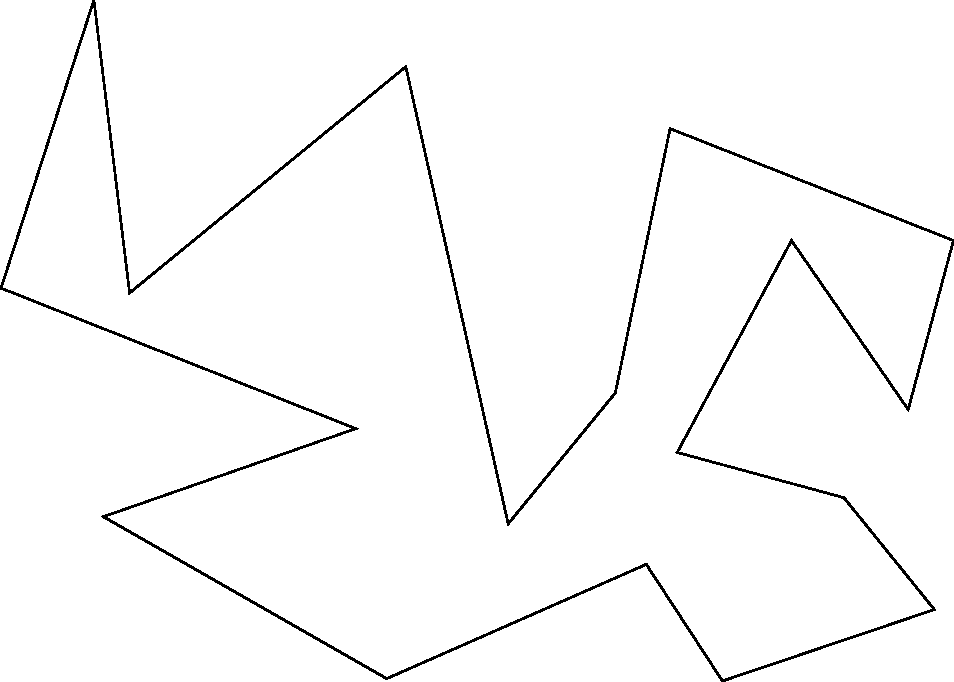
\includegraphics[height=0.3\linewidth]{obrazky-figures/Triangulacia/TriangulaciaPolygonu_pred.pdf}}\quad
\tmpframe{\includegraphics[height=0.3\linewidth]{obrazky-figures/Triangulacia/TriangulaciaPolygonu_po.pdf}}
\caption{Triangulácia polygónu metódou rezania uší. \textbf{Vľavo} sa nachádza spracovávaný mnohouholník a \textbf{vpravo} vytvorená sieť trojuholníkov.}\label{fig:triangluacia}
\end{figure}

\begin{algorithm}[H]
\caption{Triangluačná metóda rezania uší}\label{Alg:Ear_Clipping_method}
\begin{algorithmic}[1]
\Function{Triangluate}{P}
\State WatchDog=PocetBodov
\While{OstavajuciPocetBodov > 2}
	\State WatchDog=WatchDog-1
    \State PosunNaDalšieBody
  \If {ŽiadnyBodVTrojuholníku \&\& JePravotočivý}
    \State ZaznamenajBody
    \State OdrežUcho
    \State WatchDog=OstávajúciPočetBodov
  \EndIf
  \If {WatchDog==0}
  	\State break
  \EndIf
\EndWhile
\EndFunction
\end{algorithmic}
\end{algorithm}

Do tohto algoritmu som pridal aj premennú watchdog, ktorá sa postupne dekrementuje až pokým sa nenájde ucho, ktoré by sa dalo odrezať. Pre túto variantu som sa rozhodol kvôli tomu, že sa často stretávam s~nedokonalými modelmi, ktoré obsahujú prekrývajúce sa úsečky a teda sa algoritmus zacykluje. Tieto nepresnosti boli často spôsobené spojením dvoch objektov v~niektorom z~3D modelovacích nástrojov.

Unity zobrazuje iba trojuholníky, ktoré sú v~smere hodinových ručičiek. My ale chceme vidieť vytvorené plátky z~oboch strán. Preto je nutné, pridať k~vytvoreným trojuholníkom aj ich opačnú verziu pomocou zmeneny poradia bodov.

\subsection{Vzdialenosť medzi prierezmi}

V~rannej dobe tvorby projektu som nechával na užívateľovi, aby nastavil vzdialenosť medzi jednotlivými prierezmi. Tento proces ale nebol dostatočne intuitívny, a preto som sa rozhodol umožniť užívateľovi definovať, aký počet rezov má byť použítý pre tvorbu prierezov. Pri generovaní som ale musel tento počet následne pretransformovať na vzdialenosť $d_{span}$. 

Najprv si zistíme body $P_{1}$ a $P_{2}$, ktoré sa pretínajú najďalej od stredu $S$ s~rezom $R$, ktorý má rovnaké natočenie ako budú mať vytvorené prierezy. Pomocou zistených vzdialeností som získal celkovú vzdialenosť a vydelil ju potrebným počtom medzier medzi rezmi $N$. Kedže ale nechceme, aby sa prierezy generovali hneď od okraja objektu, tak je treba zinkrementovať počet medzier medzi rezmi o~jeden a tým zabezpečiť, aby sa na okraji objektu vynechal priestor rovný polovici vzdialenosti medzi prierezmi $\frac{d_{span}}{2}$.


\begin{equation}d_{span} = \frac{d_{P_{1}P_{2}}}{N + 1}
\label{eqn:span}
\end{equation}



\subsection{Posuv rezov}
Keďže použitý algoritmus generuje prierezy od stredu objektu, tak pri párnom počte by neboli prierezy rozložené rovnomerne. Kvôli tomu je nutné posunúť počiatočný prierez o~polovicu vzdialenosti medzi rezmi a zabezpečiť tak rovnomernosť vygenerovaných prierezov.

%Kedže pri párnom počte prierezov, sa prvý prierez nemá generovať od stredu objektu, musíme posunúť počiatočný prierez o polovicu vzdialenosti medzi rezmi a tým zaistiť aby sa prierezy generovali rovnomerne. 



%$$$$$$$$$$$$$$$$$$$$$$$$$$$$$$$$$$$$$$$$$$$$$$$$$$$$$$$$$$$$$$$$$$$$$$$$$$$$$$
\section{Tvorba zárezov do jednotlivých prierezov}
Na to, aby sa dali skladačky Sliceforms skladať, musíme do jednotlivých plátkov urobiť zárezy v~mieste, kde sa plátky stretávajú s~priečnymi plátkami.
Tieto zárezy musíme vytvoriť tak, aby boli do polovice celej pretínacej vzdialenosti.

Najprv musíme nájsť všetky body, v~ktorých sa pretína polygón s~kolmím plátkom. Na obrázku \ref{fig:TvorbaZarezov} máme mnohouholník $P = \{A, B, C, D, E, F, G, H\}$, ktorý pretína rovina $R$. Táto rovina pretína polygón cez päť úsečiek. Spracovanie týchto úsečiek si rozdelíme na tri časti.
\begin{itemize}
\item Úsečku $[A, B]$ pretína rovina medzi bodmi $A$ a $B$. Zaznamenáme si tento bod pretnutia.
\item Úsečku $[C, D]$ a úsečku $[D, E]$ pretína rovina práve v~jednom bode, a tým je bod $D$. Keďže body $C$ a $E$ sa nachádzajú na rovnakej strane roviny, zaznamenáme bod $D$ dvakrát, ako keby rovina pretínala úsečky niekde medzi bodmi.
\item Posledná tretia varianta spracovania je pre úsečky, ktoré rovina pretína práve v~jednom bode a zároveň sú ďaľšie doby úsečiek na rôznych stranách roviny. V~prípade mnohouholníka $P$ sú to úsečky $[F, G]$ a $[G, H]$. Rovina prechádza práve cez bod $G$, a body $F$ a $H$ sú na rôznych stranách roviny. V~tejto variante zaznamenávame spoločný bod $G$ iba raz.
\end{itemize}
To, či sú body na rovnakej alebo rozličnej strane, zisťujeme pomocou vypočítania vzdialenosti bodu od roviny, ktorej sme sa venovali v~časti \ref{Sec:Vzdialenost}. Ak majú vypočítané vzdialenosti rovnaké znamienka, spracovávame ich podľa druhej varianty. Ak majú rôzne znamienka, spracovávame ich podľa tretej varianty.


\begin{figure}[!h]
\centering
\tmpframe{\includegraphics[width=8cm]{obrazky-figures/Tvorba/tvorba_zarezov2.pdf}}
\caption{Tento obrázok zobrazuje pretnutie mnohouholníka rovinou. Rovina pretína mnohouholník práve v~troch bodoch, a to na úsečke [AB], v~bode $D$ a v~bode $G$.}
\label{fig:TvorbaZarezov}
\end{figure}

Ako prvé čo musíme urobiť je, že si nájdené body musíme zoradiť, kedže pri väčšine mnohouholníkov nevieme, ktorou úsečkou sa hľadanie začalo a nájdené body môžu byť v~zlom poradí. Keď už máme body nájdené a zoradené, môžeme začať vyznačovať zárezy. Zárezy v~$X$-ovej osi musia byť opačne ako zárezy v~$Y$-ovej osi.
Pri vyznačovaní zárezov berieme body po dvoch. Postupne spájame jeden z~týchto bodov podľa toho, v~ktorej osi zárezy robíme, s~bodom, ktorý sa nachádza práve v~strede medzi týmito dvoma bodmi. S~týmto postupom docielime, že sa nám správne vyznačia zárezy, aby sme mohli výsledný objekt správne vystrihnúť a poskladať.

%$$$$$$$$$$$$$$$$$$$$$$$$$$$$$$$$$$$$$$$$$$$$$$$$$$$$$$$$$$$$$$$$$$$$$$$$$$$$$$
\section{Finálny produkt} \label{sec:finalProduct}
%\todo{popisat o ukladani - 4 spôsoby, o ukladani do pdf a pouzitom pdfcreatore}

Aby sa vytvorený prierezový model dal použiť ako vystrihovačka, musel som vymyslieť ako ho uložiť, aby sa dal vytlačiť a vystrihnúť. Navrhol som päť možností, ktoré sa rozdeľujú do troch tried. Sú to:
\begin{description}
\item[Modelové:] Model sa uloží do súboru OBJ, a každý prierez sa uloží ako samostatný objekt. Túto možnosť som zvolil kvôli tomu, aby si užívateľ mohol danú vystrihovačku ešte pozrieť a použiť ako prípadnú pomôcku pri skladaní.
\item[Vektorové:] Vo formáte SVG alebo PDF. Pri SVG sa ukladá každý prierez do samostatného súboru. Pri PDF sa uložia všetky prierezy do jedného súboru, kde sa poukladajú podľa užívateľom zvoleného rozloženia prierezov na daný rozmer strany. Možnosť ukladania do PDF je preferovaná, keďže sa dá bez ďalších úprav hneď vytlačiť pomocou tlačiarne.
\item[Rastrové:] Pri tejto možnosti sa nám najprv vytvoria textúry, na ktoré sa vykreslia plátky. Každá z~jednotlivých textúr sa uloží do samostatného súboru a to vo formáte JPG alebo PNG. Pre jednoduchšiu manipuláciu s~vytvorenými súbormi som zvolil jednotný rozmer tvorených textúr.
\end{description}

\subsection{Ukladanie do PDF} \label{sec:PDFcreator}
Pri formáte PDF bolo nutné zvoliť si nástroj na tvorenie súborov. Našiel som niekoľko nástrojov kde väčšina pracovala s~.NET 4,0 ale kedže herný engine používa iba .NET 3,5 tak som ich nemohol použiť. Nakoniec som sa dostal k~dvom nástrojom a to SharpPdf\footnote{http://sharppdf.sourceforge.net/} a iTextSharp\footnote{http://itextpdf.com/}. 

\begin{description}
\item[SharpPdf:] Tento nástroj som používal ako prvý. Umožňuje vytvárať veľmi primitívne dokumenty. 
Hlavným prvkom je objekt pdfDokument, na ktorý sa postupne pridávajú objekty pdfPage, na ktoré sa dá písať text alebo vykreslovať jednoduché tvary ako čiary, obdĺžniky a kruhy.

\item[iTextSharp:]{ iTextSharp umožňuje oproti SharpPdf vytvárať komplexnejšie dokumenty. Hlavnou výhodou pre mňa bolo, že dokáže vykreslovať mnohouholníky, ktoré sa dajú následne vyplniť zvolenou farbou.

}
\end{description}

% V následovnej ukážke môžeme vidieť porovnanie algoritmu SharpPdf \ref{Alg:SharpPdf} a algoritmu iTextSharp \ref{Alg:iTextSharp}. V oboch prípadoch sa vytvorí dokument vo formáte PDF ktorý obsahuje dve strany o veľkosti A4. Na prvej strane je napisany text na pozicii $[50:50]$ vo veľkosti dvanástich bodov a na druhej strane je obdĺžnik s rozmerom $200v\times300\check{s}$.

% \begin{algorithm}
% \caption{Tvorba dokumentu pomocou SharpPdf}\label{Alg:SharpPdf}
% \begin{algorithmic}[1]
%   \Function{CreatePDF}{}
%   \State pdfDocument myDoc = new pdfDocument("NameOfDoc", "Author");
%   \State pdfColor color = pdfColor.Black;
%   \State pdfPage Page = myDoc.addPage(842, 595);
%   \State Page.addText("text", 50, 50, myDoc.getFontReference("Helvetica"), 12);
%   \State pdfPage Page2 = myDoc.addPage(842, 595);
%   \State Page2.drawRectangle(0,0, 200, 300, new pdfColor(1, 1, 1), color);
%   \State myDoc.createPDF(File);
%   \EndFunction
% \end{algorithmic}
% \end{algorithm}

% \begin{algorithm}
% \caption{Tvorba dokumentu pomocou iTextSharp}\label{Alg:iTextSharp}
% \begin{algorithmic}[1]
  
%   \Function{CreatePDF}{}
%   \State Document document = new Document(PageSize.A4, 0, 0, 50, 50);
%   \State \textbf{FileStream fs} = \textbf{new FileStream}(File, \textbf{FileMode}.Create);
%   \State \textbf{PdfWriter} writer = \textbf{PdfWriter}.GetInstance(document, fs);
%   \State document.Open();
%   \State cb.SetRGBColorStroke(0,0,0);
%   \State cb.BeginText();
%   \State BaseFont font = BaseFont.CreateFont();
%    \State     cb.SetFontAndSize(font, 12);
%    \State     cb.SetTextMatrix(50,50);
%    \State     cb.ShowText("text");
%    \State     cb.EndText();
  
%   \State myDoc.NewPage();
%   \State cb.Rectangle(0, 0, 200, 300);
%   \State cb.Stroke();

%   \State document.Close();
%   \State writer.Close();
%   \State fs.Close();
%   \EndFunction
% \end{algorithmic}
% \end{algorithm}

%%%%%%%%%%%%%%%%%%%%%%%%%%%%%%%%%%%%%%%%%%%%%%%%%%%%%%%%%%%%%%%%%%%%%%%%%%%
%%%%%%%%%%%%%%%%%%%%%%%%%%%%%%%%%%%%%%%%%%%%%%%%%%%%%%%%%%%%%%%%%%%%%%%%%%%
%%%%%%%%%%%%%%%%%%%%%%%%%%%%%%%%%%%%%%%%%%%%%%%%%%%%%%%%%%%%%%%%%%%%%%%%%%%
%%%%%%%%%%%%%%%%%%%%%%%%%%%%%%%%%%%%%%%%%%%%%%%%%%%%%%%%%%%%%%%%%%%%%%%%%%%
\chapter{Návrh užívateľského rozhrania}
Každá aplikácia potrebuje komunikovať s~užívateľom. 
Na to slúži užívateľské rozhranie, pomocou ktorého si užívateľ definuje v~akom natočení majú byť prierezy robené a počet rezov. Užívateľské rozhranie bolo implementované v~spolupráci s~užívateľmi. Každá časť užívateľského rozhrania bola otestovaná na užívateľoch.


\begin{figure}[!h]
\centering
\tmpframe{\includegraphics[width=0.8\linewidth]
{obrazky-figures/GUI/Screenshot_2.png}}
\caption{Na obrázku sa nachádza okno aplikácie, na ktorom je vidno použité užívateľské rozhranie.}
\label{fig:screenshot}
\end{figure}

Výzor užívateľského rozhrania môžeme vidieť na obrázku \ref{fig:screenshot}. V~strede obrazovky sa nachádzajú dve rezné plochy - jedna pre každú os. Po načítaní objektu sa na tomto mieste zobrazí zvolený objekt, u~ktorého je možné vidieť iba vnútornú stranu objektu. Aby si užívateľ vedel daný objekt lepšie predstaviť, vytvoril som náhlad, ktorý sa nachádza v~ľavej hornej časti okna.

Na pravej strane okna sa nachádza panel nastavení. Tento panel obsahuje dva panely, pomocou ktorých je možné nastaviť počet tvorených prierezov alebo rozmer, ktorý bude použitý na tvorbu prierezov. Tento panel môžeme vidieť aj na obrázku \ref{fig:Xaxis}.  Pomocou tohto panela si môže užívateľ zvoliť natočenie reznej plochy a aj prípadný posuv. Ďalej si v~tomto panely môže zmeniť farbu vytváraných prierezov a pomocou prepínača môže vytvorené prierezy v~danej osi skryť.

\begin{figure}[!h]
\centering
\tmpframe{\includegraphics[width=0.4\linewidth]
{obrazky-figures/GUI/X-panel-count.png}}\quad
\tmpframe{\includegraphics[width=0.4\linewidth]
{obrazky-figures/GUI/X-panel-span.png}}
\caption{Panel pre nastavenie tvorby rezov. \textbf{Vľavo} je pre nastavenie počtu tvorených rezov a \textbf{vpravo} je pre nastavenie rozmeru medzi tvorenými plátkami.}
\label{fig:Xaxis}
\end{figure}


Na spodnej časti panela nastavení sa nachádzajú tlačidlá pre zobrazenie panela na zvolenie súboru a panel na uloženie vytvorených plátkov. Taktiež sa tu nachádza aj tlačidlo pre~tvorbu prierezov a tlačidlo, pomocou ktorého sa vytvorené plátky zmažú.
Tlačidlo pre~ukladanie sa sprístupní užívateľovi až po vytvorení prierezov a tlačidlo pre~tvorbu prierezov sa sprístupní až po zvolení objektu na~spracovanie. Pri sprístupnení sa zmení farba tlačidla. Toto opatrenie som zvolil kvôli zjednodušeniu užívateľského rozhrania, kde užívateľ stále vie, aké operácie sú prístupné.








%\section{Color picker}
Užívateľovi tiež umožňujem vybrať aj v~akej farbe sa plátky zobrazia. Na tento účel som vytvoril jednoduchý panel na výber farby (color picker), ktorý môžeme vidieť na obrázku \ref{fig:colorPicker}.
%Tento color picker sa otvorý po kliknutí na 
Na tomto panely sa nachádzajú tri posuvníky (slider), pomocou ktorých si užívateľ môže zvoliť veľkosť červenej, zelenej a modrej zložky farby. 

\begin{figure}[H]
\centering
\tmpframe{\includegraphics[width=0.4\linewidth]
{obrazky-figures/GUI/ColorPicker.png}}\quad
\caption{Panel pre zvolenie farby}
\label{fig:colorPicker}
\end{figure}

%\section{File explorer}

Vytvoril som aj jednoduchý prehliadač súborov (file explorer), ktorý môžeme vidieť na~obrázku \ref{FileExplorer}. Pomocou tohto prehliadača môže užívateľ prechádzať súbory a vybrať súbor vo~formáte OBJ, ktorý sa bude spracovávať, prípadne zvoliť si cestu pre uloženie vytvorených plátkov do súboru. 

V~panely ukladania môže užívateľ vybrať v~akom formáte chce vytvorené plátky uložiť. Tieto možnosti sme si prešli v~časti \ref{sec:finalProduct}. Pri súborovom formáte PDF si môže užívateľ zvoliť veľkosť papiera (A5, A4, A3) a rozloženie v~akom budú plátky uložené na papieri. Umožňujem sedem možností rozloženia, a to $1\times1$, $1\times2$, $2\times3$, $3\times4$, $4\times5$, $4\times6$ a $5\times7$.
Ďalej si môže užívateľ zvoliť obvodovú farbu, a to či sa plátky vyplnia vybranou farbou, ktorou boli vytvorené alebo či ostanú bez výplne. 
Ukladanie sa spracováva pomocou nástroja na~vytváranie pdf súborov, ktorému sme sa venovali v~časti \ref{sec:PDFcreator}.

\begin{figure}[!h]
\centering
\tmpframe{\includegraphics[width=0.4\linewidth]
{obrazky-figures/GUI/LoadPanel.png}}\quad
\tmpframe{\includegraphics[width=0.4\linewidth]
{obrazky-figures/GUI/SavePanel.png}}
\caption{\textbf{Vľavo} je panel pre zvolenie súboru vo formáte OBJ a \textbf{vpravo} je panel pre uloženie vytvorenej vystrihovačky.}
\label{FileExplorer}
\end{figure}


Aplikácia sa dá ovládať aj prostredníctvom klávesnice a myšky. Aplikácia umožňuje užívateľovi zobraziť obvodovú čiaru okolo vytvorených plátkov. Pomocou tejto obvodovej čiary je možné lepšie vidieť jednotivé plátky a pri skrytí niektorej z~osí je možné vidieť aj vytvorené zárezy. Táto funkcia sa zapína klávesmi \texttt{Ctrl} a \texttt{Q}. V~aplikácii je možné prepínať medzi zobrazením v~okne alebo zobrazením na celú obrazovku pomocou kláves \texttt{Ctrl} a \texttt{F}. Ďaľšie nastavenie, ktoré aplikácia umožňuje, je zmena osvetlovania načítaného objektu pomocou kláves \texttt{Ctrl} a \texttt{E}. Osvetlenie objektu sa prepína medzi svetlom z~kamery, svetlom krúžiacim okolo objektu a statickým svetlom. Kameru je možné ovládať myšou, šípkami alebo numerickou klávesnicou.
Aplikáciu je možné vypnúť pomocou klávesy \texttt{Esc}.

Tieto možnosti ovládania s~klávesami sú užívateľovi zdelené v~ľavom hornom rohu, kde sa pomocou klávesy \texttt{M} zobrazia aj klávesy použiteľné k~ovládaniu kamery.

%%%%%%%%%%%%%%%%%%%%%%%%%%%%%%%%%%%%%%%%%%%%%%%%%%%%%%%%%%%%%%%%%%%%%%%%%%%
%%%%%%%%%%%%%%%%%%%%%%%%%%%%%%%%%%%%%%%%%%%%%%%%%%%%%%%%%%%%%%%%%%%%%%%%%%%
%%%%%%%%%%%%%%%%%%%%%%%%%%%%%%%%%%%%%%%%%%%%%%%%%%%%%%%%%%%%%%%%%%%%%%%%%%%
%%%%%%%%%%%%%%%%%%%%%%%%%%%%%%%%%%%%%%%%%%%%%%%%%%%%%%%%%%%%%%%%%%%%%%%%%%%
\chapter{Experimentálne vyhodnotenie vytvoreného riešenia}

Ako prvé som sa rozhodol skladať iba jednoduché objekty. Ako prvý objekt som poskladal truhličku \ref{Truhlicka}. Táto skladačka bola vytvorená iba z~obyčajného kancelárskeho papiera (80g), ktorý je veľmi mäkký, a preto vytvorený model je veľmi labilný. Bolo ťažké skladať túto skladačku aj keď je tvorená iba z~ôsmich rezov a bola vytlačená vo veľkosti formátu A5.

\begin{figure}[!h]
\centering
\tmpframe{\includegraphics[height=0.4\linewidth]{obrazky-figures/CreatedObjects/truhlicka/truhlicka.pdf}}\quad
\tmpframe{\includegraphics[height=0.4\linewidth]{obrazky-figures/CreatedObjects/truhlicka/Screenshot.png}}
\caption{Truhlička. \textbf{Vľavo} je v~skutočnosti a \textbf{vpravo} v~programe.}
\label{Truhlicka}
\end{figure}

Ako ďalší objekt som poskladal guľu \ref{fig:gula} a cubotahedron \ref{fig:cubotahedron}, čo je v~podstate kocka s~odrezanými vrcholmi. Tieto objekty sú poskladané z~farebného papiera s~gramážou 225g. Pri guli boli zárezy tvorené jedným zastrihnutím do prierezu v~strede vyznačenej plochy. Táto skladačka sa veľmi ťažko skladala, pretože takto vytvorené zárezy sú veľmi úzke a teda priestor v~záreze nebol dostatočný pre vkladané prierezy. Tento objekt sa po zložení stále zmršťoval a bolo treba jemné tlačenie na hrany, inak by nepripomínal guľu ale skôr vajce. Pri~cubotahedrone bolo do každého zárezu zastrihnuté dvakrát, ako je uvedené na~obrázku \ref{fig:zastrihovanie}. Bolo oveľa jednoduchšie skladať túto skladačku a výsledný objekt si držal aj svoj pôvodný tvar. 


\begin{figure}[!h]
\centering
\tmpframe{\includegraphics[height=0.4\linewidth]{obrazky-figures/CreatedObjects/gula.pdf}}\quad
\tmpframe{\includegraphics[height=0.4\linewidth]{obrazky-figures/CreatedObjects/gula2.pdf}}
\caption{Guľa}\label{fig:gula}
\end{figure}

\begin{figure}[!h]
\centering
\tmpframe{\includegraphics[height=0.4\linewidth]{obrazky-figures/CreatedObjects/cubotahedron1.pdf}}\quad
\tmpframe{\includegraphics[height=0.4\linewidth]{obrazky-figures/CreatedObjects/cubotahedron2.pdf}}
\caption{Cubotahedron}\label{fig:cubotahedron}
\end{figure}

Po vytvorení týchto jednoduchých objektoch som sa rozhodol pre vytvorenie zložitejšieho modelu a to modelu gumennej kačičky, ktorý môžeme vidieť na obrázku \ref{fig:duck}.
\begin{figure}[!h]
\centering
\tmpframe{\includegraphics[height=0.4\linewidth]{obrazky-figures/CreatedObjects/Duck/duck.pdf}}\quad
\tmpframe{\includegraphics[height=0.4\linewidth]{obrazky-figures/CreatedObjects/Duck/duck2.pdf}}
\caption{Gumená kačička}\label{fig:duck}
\end{figure}
\section{Označenie zárezov}
Pri skladaní prvých objektov som zistil, že je veľmi náročné pre užívateľa začať skladať keď nevie, do ktorého zárezu má ísť ktorý plátok. Preto som sa rozhodol pridať pomôcku pre skladajúceho a označiť jednotlivé zárezy indexom prierezu. Výslednú ukážku je možné vidieť na obrázku \ref{fig:OznaceneZarezy}.
\begin{figure}[!h]
\centering
\tmpframe{\includegraphics[width=8cm]{obrazky-figures/zarezy.pdf}}
\caption{Ukážka výsledného rezu s~označením zárezov v~pdf}
\label{fig:OznaceneZarezy}
\end{figure}

\section{Výkonový test}
\begin{figure}[!h]
\centering
\tmpframe{\includegraphics[width=12cm]{obrazky-figures/gule.png}}
\caption{Objekt gule použitý na test}
\label{fig:Gule}
\end{figure}
Na zaznamenanie doby výpočtu bol použitý objekt gule, v~ktorej bol navyšovaný počet plôch v~stĺpcoch a riadkoch. Tieto modely môžeme vidieť na obrázku \ref{fig:Gule}. Guľu som si vybral preto, že je vždy konvexná a teda je doba generovania viac zameraná na tvorbu prierezov a zárezov do nich a nie na použitý triangulátor. K~testovanému modelu bolo postupne pridávaných 5 riadkov a 5 stĺpcov. Výsledok tohto testu je zobrazený na grafe \ref{fig:grafCasGenerovania}. 
\begin{figure}[!h]
\centering
\tmpframe{\includegraphics[width=15cm]{obrazky-figures/GrafCasGenerovania.pdf}}
\caption{Doba generovania skladačky Sliceform}
\label{fig:grafCasGenerovania}
\end{figure}

\chapter{Záver}
%Cieľom tejto práce bolo navrhnúť a vytvoriť jednoduchú aplikáciu na tvorbu skladačiek Sliceforms.
%Táto práca sa začína opisom týchto skladačiek a ich skladaním. Nasleduje reprezentácia geomotrických telies v počítačovej grafike a pokračuje možnými problémami pri ich tvorbe.

V~tejto práci som popísal vystrihovačky Sliceforms aj s~matematikou a geometriou na ich tvorbu.
Tento nástroj na tvorbu skladačiek som v~práci navrhol a následne aj implementoval v~hernom jadre Unity.

Táto aplikácia vytvorí prierezy podľa užívateľom definovaného natočenia a posuvu zo~zadaného polygonálneho objektu. Do týchto vytvorených prierezov vytvorí zárezy v~mieste, kde sa plátky pretínajú s~kolmými plátkami. Tieto vytvorené plátky si môže užívateľ pozrieť v~3D priestore a následne uložiť do niektorého z~dostupných súborových formátov. Vytvorený nástroj aj s~užívateľským rozhraním bol konzultovaný a testovaný na užívateľoch. Ako som na konci práce ukázal, po vytlačení na papier a následnom vystrihnutí si môže užívateľ vytvorenú skladačku aj poskladať. 

%V budúcnosti by som chcel pokračovať v tejto práci. 

Je niekoľko možností ako aplikáciu vylepšiť. Napríklad by si aplikácia sama zvolila optimálne rozloženie prierezov tak, aby 
%...
bolo 
%robených...
viac prierezov v~užších miestach a v~širších miestach menej. Poprípade by umožnila užívateľovi upraviť rozloženie prierezov tak, aby si mohol ľubovoľne zmeniť jednotlivé rozostupy medzi vybranými rezmi.






%=========================================================================
